\chapter{Basic Concept}
\setlength{\parskip}{1em} 

\section{Laser Engraving}
Laser engraving is a subtractive process that uses a focused laser beam to remove material from a surface, creating permanent marks without physical contact or tool wear. There are two principal techniques to generate these engravings: vector engraving and raster engraving. \cite{HaiTechLasers:MasterGuideLaserEngraving}

\begin{itemize}
	\item \textbf{Vector Engraving:} It relies on drawing continuous paths along predefined shapes, such as lines, curves, or outlines as shown in the figure ~\ref{vector}. The laser follows these vector paths directly, similar to how a pen moves when drawing. This method is efficient for simple geometries such as borders, logos, or line art, but becomes less suitable for dense areas of filled text or images. \cite{CNCSourced:RasterVsVectorEngravingGuide} \cite{xTool:RasterVsVectorEngraving}
	
	
	\item \textbf{Raster Engraving:} by contrast, treats the design as a pixel-based image. The laser scans the surface line by line (similar to the operation of an inkjet printer), switching between ON and OFF states according to the black-and-white pattern of the image as shown in the figure ~\ref{raster}. This method is more appropriate for detailed text, photographs, or shaded regions, where filled areas need to be represented precisely. \cite{CNCSourced:RasterVsVectorEngravingGuide} \cite{xTool:RasterVsVectorEngraving}
	
\end{itemize}

\noindent
\begin{minipage}{0.45\textwidth}
	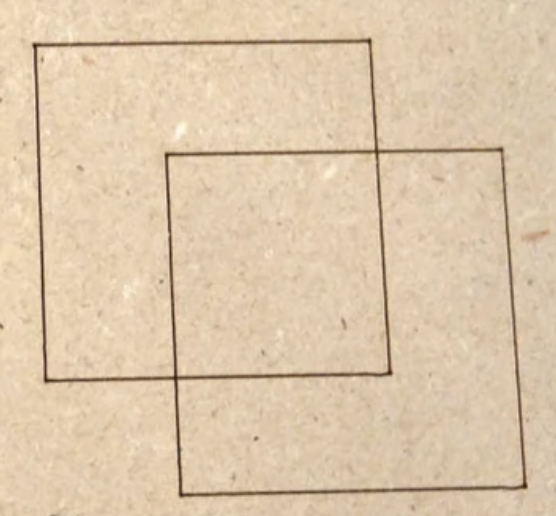
\includegraphics[width=\linewidth]{Images/vector.png}
	\centering
	\captionof{figure}{Vector Engraving} 
	\label{vector} 
\end{minipage}
\hfill
\begin{minipage}{0.45\textwidth}
	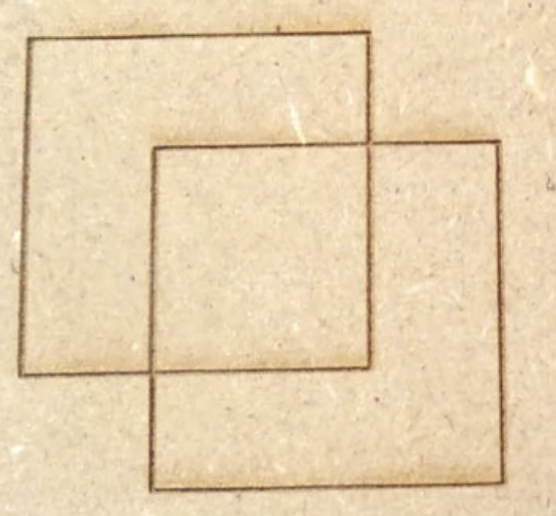
\includegraphics[width=\linewidth]{Images/raster.png}
	\centering
	\captionof{figure}{Raster Engraving}
	\label{raster}
\end{minipage}

	A widely used method in raster engraving is the scanline principle, whereby the laser head moves consistently across each row (scanline) and shifts down incrementally after each pass. It delivers high fidelity engraving of detailed images or filled patterns, though it is typically slower compared to vector engraving. \cite{OneLaser:RasterVsVectorEngraving}

	Raster engraving is especially apt for business card reproduction, capturing intricate details like logos, text, and QR codes with high accuracy, whereas vector engraving may only be practical for outlining or borders. By combining both methods, the system achieves both precision and flexibility, accommodating complex visual content and simple line art alike.
	
\section{Core Concepts}

\subsection{Optical Character Recognition (OCR)}
OCR converts images of printed or handwritten text into machine-readable text, enabling digital editing, indexing, or downstream processing.

In this project, OCR extracts name, contact details, and address from the scanned card. Preprocessing ensures clean input, while post-processing (e.g., pattern‑based classification) groups text into semantic categories like "email" or "phone", which is a method commonly used in business card recognition tools. \cite{MadanKumar:BusinessCardOCR2019}

\subsection{Computer Vision \& Layout Detection}
Beyond raw text extraction, correctly identifying regions such as logos or QR codes relies on layout detection and classification. Vision‑language models like Qwen2.5‑VL can detect and localise multiple heterogeneous elements in a single pass. This object‑level detection ensures that visual components are correctly distinguished before vectorisation. \cite{Wikipedia:DocumentLayoutAnalysis}

Our system, layout analysis ensures that each detected element is recognized and mapped to accurate positions in the SVG design, which is essential for precise engraving control. 

\subsection{Scalable Vector Graphics (SVG)}
SVG is an XML-based vector image format representing graphics as scalable paths and shapes, ideal for precise positioning and editing.

SVGs are pivotal in our project because they preserve resolution independence and allow command-based or natural-language editing before engraving. Recent research demonstrates how modern models can generate high-quality and semantically-rich SVGs directly from images or text. \cite{StarVector:Arxiv2312.11556v4}

\subsection{Rasterisation and Binarisation}
Rasterisation converts vector graphics into pixel-based images, while binarisation reduces them to black-and-white bitmaps suitable for laser engraving. These steps ensure high-contrast and noise-free imagery optimising it for scanline‑based laser execution.

\subsection{G-code Generation}
G-code is a numerical control language for directing machine tool movement (e.g., lasers or 3D printers). In laser engravers it instruct how to move and when to toggle the laser. It includes commands like G0 (rapid move) and G1 (controlled engraving move) define the path and engraving speed, while laser activation (e.g., M3, S) controls intensity. \cite{Yang:SVGtoGcode2021}

In our implementation, a scanline algorithm parses raster bitmaps into efficient G-code sequences. The generated G-code enables control over movement and laser intensity, followed by a preview for validation before actual engraving.

	
\section{System Data Flow}

The system’s data flow outlines the sequential transformation from a photographed business card to laser-ready G-code. Structuring the workflow in clearly defined stages ensures both modularity and interpretability—principles central to robust system design in automation contexts.

\subsection{Overview of the Pipeline}
The system follows a structured, multi-stage process:

\begin{itemize}
	\item \textbf{Image Acquisition:} Capture or obtain a digital image of the business card.
	\item \textbf{OCR \& Layout Detection:} Visual content—including text, logos, QR codes, and embedded elements, is detected using OCR and vision-language models, which provide semantic and positional information. These models increasingly replace multi-step pipelines by combining detection and recognition in one pass.
	\item \textbf{SVG Synthesis:} Detected elements are rendered into an SVG format, respecting physical dimensions (e.g., 85 $\times$ 54 mm) and spatial relationships. SVG’s vector nature ensures scale independence and editing flexibility.
	\item \textbf{Optional Editing:} Users may adjust the design via structured commands or natural language through an LLM, ensuring human oversight while preserving automation.
	\item \textbf{Rasterization and Binarization:} The SVG is converted into a high-contrast black-and-white bitmap, suitable for precise laser engraving.
	\item \textbf{G-code Generation:} Using a scanline strategy, the raster image is translated into G-code (e.g., G0/G1 commands with laser ON/OFF), encoding laser movement and power control.
	\item \textbf{Preview \& Execution:} A visual preview of the G-code toolpath is rendered for validation before being sent to the Laser Engraver Module in the Digital Factory.
\end{itemize}

\subsection{Diagrammatic Representation}

\begin{figure}
	\begin{center}
		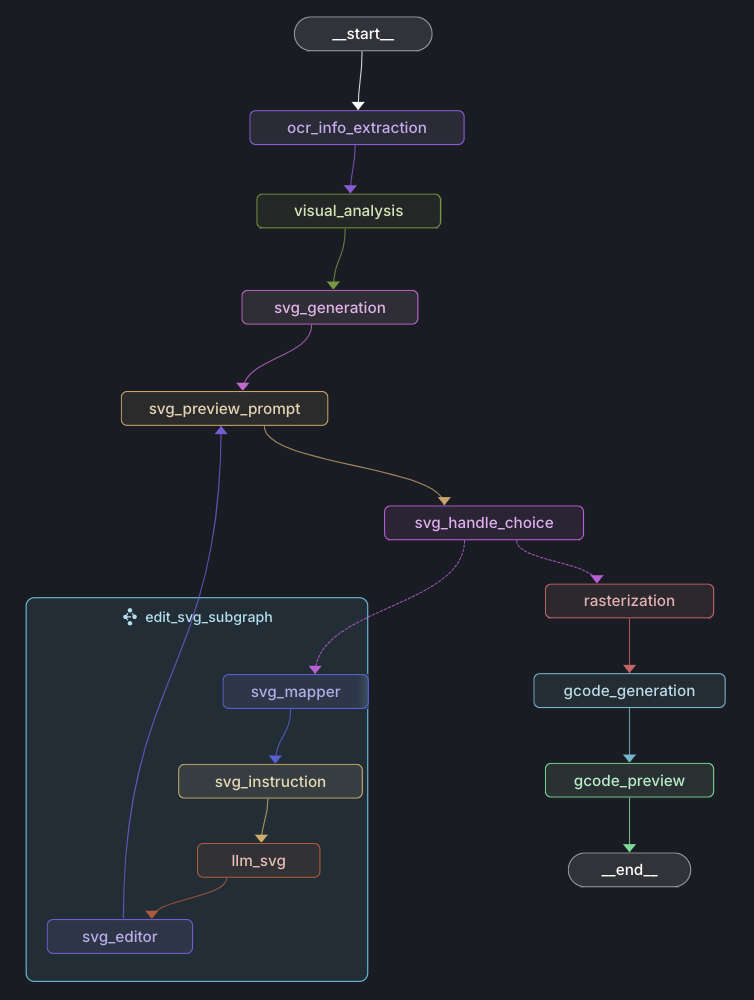
\includegraphics[width=0.6\linewidth]{Images/Langgraph.png}
		\caption{Langgraph Workflow}
		\label{Langgraph} 
	\end{center}
\end{figure}

Above, you’ll see an illustrative pipeline diagram ~\ref{Langgraph} that represents this workflow:


\begin{itemize}
	\item \textbf{Start:} Business card image input
	\item \textbf{Next:} OCR \& layout detection
	\item \textbf{Then:} SVG generation → optional editing
	\item \textbf{Following:} Rasterization → binarization
	\item \textbf{Then:} G-code generation
	\item \textbf{End:} Preview → Laser engraver
	
\end{itemize}
		
	This diagram helps readers visualize how data transitions across stages and underscores the modular orchestration via agent-based design.
	
	
\section{Agents \& LangGraph Orchestration}

In modern AI systems, particularly those involving sequential or multi-step tasks, it's advantageous to structure the workflow as a collection of specialized agents, each responsible for a well-defined task, rather than a monolithic process. This modular approach enhances clarity, maintainability, and scalability, while enabling dynamic control flows and human oversight. \cite{Chase:ThinkAboutAgentFrameworks2025}

\subsection{Agents and Workflow Decomposition}

An agent in this context is an autonomous component—often powered by a large language model, that processes input, performs a task, and passes output forward. Multi-agent architectures allow \cite{Chase:ThinkAboutAgentFrameworks2025}:

\begin{itemize}
	\item \textbf{Specialization:} Each agent focuses on a single responsibility, improving clarity and testability.
	\item \textbf{Modularity:} Agents can be developed, tested, and iteratively improved in isolation.
	\item \textbf{Controlled orchestration:} The flow between agents can be governed dynamically, based on state or external feedback, facilitating flexibility in the face of uncertain inputs
\end{itemize}


\subsection{Introduction to LangGraph}
LangGraph is a graph-based orchestration framework built to manage agentic systems. It combines declarative graph definitions with imperative node logic, enabling both predictability and flexibility. Key features include:
\begin{itemize}
\item \textbf{Nodes} represent discrete agent tasks or decision points
\item \textbf{Edges} define transitions, which can be condition-driven.
\item \textbf{State persistence} allows workflows to pause, resume, or even support \textbf{human-in-the-loop} interventions, making it applicable to interactive systems where approval or corrections may be necessary.
\item LangGraph supports \textbf{streaming updates}, memory handling, and integrates with tools like LangSmith for debugging and visualization.
\end{itemize}

\subsection{Application in our Project}
This project leverages the agentic paradigm and LangGraph orchestration, fig. ~\ref{Langgraph} to construct a clean, modular pipeline:

\begin{itemize}
	\item \textbf{OCR Agent:} Extracts textual information from the input image.
	\item \textbf{Visual Analysis Agent:} Detects layout elements like logos, QR codes, and text blocks.
	\item \textbf{SVG Generation Agent:} Assembles detected components into an editable vector design.
	\item \textbf{Editing Agent (LLM-SVG):} Receives human or language-based inputs to adjust layout or content.
	\item \textbf{Rasterisation Agent:} Converts SVG to a clean, black‑and‑white bitmap.
	\item \textbf{G‑code Agent:} Translates scanlines into laser movement instructions.
	\item \textbf{Preview Agent:} Generates a visual tool‑path preview for validation.
\end{itemize}

Each agent processes only its designated output and hands off structured state to the next, following the pipeline-of-agents pattern \cite{Honchar:PipelineOfAgents2025}. This design allows:
\begin{itemize}
\item \textbf{Isolated development and debugging} of agents.
\item \textbf{Human oversight} at the SVG editing or preview stages.
\item \textbf{Stateful execution} the workflow can pause for edits or resume after failures.
\item \textbf{Traceability} the graph structure enables clear tracking of data and decisions across stages.
\end{itemize}

\subsection{Benefits}

Using LangGraph orchestration in this project provides specific advantages for automating the laser engraving pipeline:
\begin{itemize}
\item \textbf{Predictability and Agency:}

The engraving pipeline requires deterministic steps (e.g., rasterisation must always follow SVG generation) but also benefits from flexible decision points (e.g., when a user chooses to edit the SVG or proceed directly to G-code). LangGraph ensures the overall flow is predictable, while still allowing human-in-the-loop interventions where agency is needed.

\item \textbf{Fault Tolerance and Robustness:}

In practice, OCR errors or misaligned layout detection can occur when processing diverse business cards. LangGraph’s persistent state allows the workflow to pause, request corrections (e.g., manual confirmation of text or layout), and then resume without restarting the entire process. This robustness is essential for maintaining accuracy across different card designs.

\item \textbf{Alignment with Agentic AI Principles:}

The project demonstrates how modular agents, OCR, visual analysis, SVG generation, editing, rasterisation, and G-code preview, can be coordinated into a coherent workflow. This mirrors current research trends in agentic AI, where specialized modules are orchestrated to solve complex, multi-step tasks reliably in industrial contexts.
\end{itemize}

\section{Key Tools and Libraries Used}

The implementation of the AI-GCode-Generation project relies on a combination of software frameworks, libraries, and AI models, each serving a specific role in the pipeline. By integrating these tools, the system achieves modularity, robustness, and adaptability within the Digital Factory’s Laser Engraver Module.

\subsection{Programming Environment}

\begin{itemize}
\item \SHELL{Python 3.12} 

The core programming language and environment for implementing the system. Python’s extensive ecosystem of libraries for computer vision, vector graphics, and machine learning makes it highly suitable for developing AI-assisted engraving workflows.

\end{itemize}

\subsection{Workflow Orchestration}

\begin{itemize}
\item \SHELL{LangGraph (langgraph-cli, langgraph-api)}

Provides the orchestration layer for structuring the pipeline into modular agents. It defines the graph-based workflow, connects nodes representing tasks (OCR, SVG generation, editing, rasterisation, etc.), and ensures predictable state transitions with support for human-in-the-loop editing. This makes the system both scalable and extensible in the context of the Digital Factory

\end{itemize}

\subsection{Computer Vision and Image Processing}

\begin{itemize}
	\item \SHELL{OpenCV (opencv-python)}
	
	Used in modules such as \texttt{visual\_analysis\_agent.py} and \texttt{rasterization.py} for image preprocessing, layout analysis, and bitmap conversion. OpenCV enables operations like contour detection, grayscale transformations, and QR code recognition.
	
	\item \SHELL{NumPy}
	
	Provides efficient array and matrix operations required in rasterisation and scanline generation. It is also used in processing pixel data before translation into G-code.
	
	\item \SHELL{Matplotlib}
	
	Applied for debugging and visual verification, e.g., plotting bounding boxes during layout analysis or displaying rasterised images before engraving.
\end{itemize}

\subsection{Vector Graphics Handling}
\begin{itemize}
	\item \SHELL{svgwrite}
	
Used in \texttt{svg\_agent.py} to generate SVG files programmatically. It enables precise positioning of text, logos, and QR/NFC elements in millimetre coordinates, ensuring layout fidelity.
	
	\item \SHELL{svgpathtools}
	
Provides geometric path manipulation for SVG elements, particularly useful when refining coordinates and handling transformations within the generated designs.
	
	\item \SHELL{CairoSVG}
	
Converts generated SVG files into PNG images, which serve as the input for binarisation and engraving preparation.

\end{itemize}

\subsection{G-code Generation}
\begin{itemize}
	\item \SHELL{svg2gcode}
	
A dedicated library that translates vector paths into G-code. In this project, it is integrated with a custom rasterisation module to produce scanline engraving paths, where the laser toggles ON for black pixels and OFF for white pixels
	
\item \SHELL{Custom G-code Generator}
	
Used in \texttt{gcode\_agent.py}, extends beyond svg2gcode by implementing raster scanline algorithms, zig-zag motion control, and feedrate tuning for the laser engraver.
	
\end{itemize}

\subsection{AI Models}
\begin{itemize}
	\item \SHELL{Qwen2.5-VL}
	
A vision-language model used in \texttt{ocr\_agent.py} and \texttt{visual\_analysis\_agent.py} to detect layout elements (logos, QR codes, NFC chips, text regions) and extract structured data such as names, phone numbers, and email addresses. This enables semantic interpretation of card images
	
\item \SHELL{Mistral 7B (via OpenRouter)}
	
Employed in \texttt{llm\_svg\_agent.py} to interpret \texttt{natural language editing commands} (e.g., “move logo to top-right” or “replace title with ‘Senior Engineer’”) and convert them into structured SVG edit instructions. This allows intuitive, user-friendly interactions
	
\end{itemize}

\subsection{User Interaction and Preview}
\begin{itemize}
	\item \SHELL{Tkinter}
	
A lightweight GUI toolkit used in \texttt{svg\_preview\_agent.py} and \texttt{gcodePreview\_agent.py}. It provides zoomable preview windows for both SVG and G-code, enabling the user to validate layouts and engraving toolpaths before final execution.
	
\end{itemize}
 
 \subsection{Supporting Libraries}
 \begin{itemize}
 	\item \SHELL{pydantic}
 	
 	Used for data validation and structured JSON handling, ensuring that extracted OCR and layout data conforms to expected formats.
 	
 	\item \SHELL{python-dotenv}
 	
 	Handles environment variables, storing API keys and configuration securely (e.g., Fireworks API for OCR, OpenRouter API for LLM).
 	
 	\item \SHELL{python-dotenv}
 	
 	Handles environment variables, storing API keys and configuration securely (e.g., Fireworks API for OCR, OpenRouter API for LLM).
 	
 	\item \SHELL{qrcode, pyzbar}
 	Support detection and embedding of QR codes in the pipeline, ensuring scannable codes are correctly reproduced on engraved cards.
 	
 \end{itemize}